%\documentclass[dvipsnames,format=sigconf,anonymous=true,review=true]{acmart}
\documentclass[dvipsnames,format=sigconf]{acmart}

\usepackage[utf8]{inputenc}

\acmDOI{10.1145/nnnnnnn.nnnnnnn} % To be updated after completing copyright process
\acmISBN{978-x-xxxx-xxxx-x/YY/MM} % To be updated after completing copyright process
\acmConference[GECCO '25]{The Genetic and Evolutionary Computation Conference 2025}{July 14--18, 2025}{Málaga, Spain}
\acmYear{2025}
\copyrightyear{2025}

\title{Energy Efficiency of C++ Standard Random Number Generators}

\author{Gustavo Romero López}
\affiliation{%
  \institution{Universidad de Granada}
  \streetaddress{Avenida del Hospicio, s/n}
  \postcode{18010}
  \city{Granada}
  \state{Andalucía}
  \country{Spain}
}
\email{gustavo@ugr.es}
\orcid{0000-0002-5498-7512}

\author{Juan Julián Merelo Guervos}
\affiliation{%
  \institution{Universidad de Granada}
  \streetaddress{Avenida del Hospicio, s/n}
  \postcode{18010}
  \city{Granada}
  \state{Andalucía}
  \country{Spain}
}
\email{jmerelo@ugr.es}
\orcid{0000-0002-1385-9741}

\begin{document}

\begin{abstract}
  Random number generation is widely used in many different algorithms, yet its inner workings and performance are poorly understood among many of its users. In this paper, we aim to explore one of its lesser-known aspects: energy consumption. Most studies on the subject tend to focus on the quality of the generators or on measuring their execution times. However, energy consumption is a critical concern today, particularly for mobile devices.

  In this work, we have measured the energy consumption of standard C++ random number generators. The results reveal differences in energy usage of over a thousand-fold, which could be significant for applications that require the generation of large quantities of random numbers, such as learning algorithms and metaheuristics.
\end{abstract}

%
% The code below should be generated by the tool at
% http://dl.acm.org/ccs.cfm
% Please copy and paste the code instead of the example below.
%
\begin{CCSXML}
<ccs2012>
   <concept>
       <concept_id>10011007.10011074.10011075.10011079.10011080</concept_id>
       <concept_desc>Software and its engineering~Software design techniques</concept_desc>
       <concept_significance>300</concept_significance>
       </concept>
   <concept>
       <concept_id>10003752.10003809.10003716.10011136.10011797</concept_id>
       <concept_desc>Theory of computation~Optimization with randomized search heuristics</concept_desc>
       <concept_significance>300</concept_significance>
       </concept>
   <concept>
       <concept_id>10003752.10003809.10003716.10011136.10011797.10011799</concept_id>
       <concept_desc>Theory of computation~Evolutionary algorithms</concept_desc>
       <concept_significance>500</concept_significance>
       </concept>
   <concept>
       <concept_id>10011007.10010940.10010941.10010949.10010957.10010964</concept_id>
       <concept_desc>Software and its engineering~Power management</concept_desc>
       <concept_significance>500</concept_significance>
       </concept>
 </ccs2012>
\end{CCSXML}

\ccsdesc[300]{Software and its engineering~Software design techniques}
\ccsdesc[500]{Theory of computation~Random search heuristics}
\ccsdesc[500]{Theory of computation~Evolutionary algorithms}
\ccsdesc[500]{Software and its engineering~Power management}

\keywords{Green computing, software engineering, evolutionary algorithms, genetic algorithms, energy-aware algorithms, RNGs}

\maketitle

\section{Introduction}
\label{sec:introduction}

Pseudo-random number generators \cite{marsaglia2003random} are a fundamental resource in computing, which is why they have been extensively studied in numerous works. However, most of these studies focus on the quality of the generated numbers or the efficiency of the algorithms that produce them. In this paper, we aim to focus on a less-studied aspect: the energy consumption of random number generators (RNGs). This aspect is critical today, especially in mobile devices, where energy consumption is a limiting factor. In this work, we have measured the energy consumption of standard C++ RNGs.

Most of them are initialized with a series of numbers used as seeds. A one-way function is then applied to these seeds, resulting in a random number. To generate a new random number, the previous one is used as the new seed and is subjected to the same process.

The properties of RNGs can vary significantly depending on the field in which they are used. For certain applications, such as cryptography, generators must pass highly rigorous quality tests, such as Diehard \cite{marsaglia1997diehard} or TestU01 \cite{testu01}. However, for many other applications, such as genetic algorithms, the generators must be fast and efficient, even at the expense of lower quality. In fact, some studies suggest that genetic algorithms are not highly sensitive to the quality of RNGs \cite{cardenas2011sensitiveness}.

\subsection{State of the art}
\label{sec:state-of-the-art}

Pseudo-random number generation is a widely studied field \cite{marsaglia2003random}. However, its practical implementation in programming languages has not been as thoroughly explored. In the language we focus on in this work, C++, the standard library provides several pseudo-random number generators, each with its own characteristics and properties. Their efficiency has only been superficially examined in online resources \cite{kd9f9-2020,arbelaez-2016}, but not in rigorous scientific articles. Moreover, the energy efficiency of these generators has not been studied at all.

On the other hand, there are numerous libraries for Genetic and Evolutionary Algorithms such as Pagmo \cite{Biscani2020}, OpenGA \cite{8122921}, ParadisEO \cite{Dreo-al_2021_Paradiseo}, GAlib \cite{wall1996galib} and PGAPack \cite{levine1996users} that make extensive use of RNGs. Most of them either use standard RNGs or their own implementations, for which there are no comparative studies on efficiency, let alone energy consumption.

Pagmo, OpenGa and ParadisEO uses the Mersenne Twister \cite{mersennetwister} as its default RNG, which is one of the most widely used RNGs in the world. However, it is not the most efficient in terms of time and energy consumption, as we will show in this work. The same can be said for the other libraries mentioned above, which use the same or similar RNGs.

GAlib and PGAPack can either use the C \texttt{rand} function or implement their own RNG as the default option. Both approaches are among the least efficient in terms of time and energy consumption, which is consistent with the results we will demonstrate in this work.

\section{Methodology and results}
\label{sec:methodology}

To measure the energy consumption of C++ RNGs, we wrote a program that generates 100 million random numbers using each of the C++ standard engines: \texttt{std::knuth\_b},  \texttt{std::minstd\_rand0} \\(\texttt{std::default\_random\_generator}),  \texttt{std::minstd\_rand}, \\ \texttt{std::mt19937}~\cite{mersennetwister},  \texttt{std::mt19937\_64}~\cite{mersennetwister}, \texttt{std::ranlux24\_base}, \texttt{std::ranlux48\_base},  \texttt{std::ranlux24}~\cite{JAMES1994111}, \texttt{std::ranlux48}~\cite{JAMES1994111}.

We also included other well-known generators, either due to their relevance, \texttt{rand} de C, their inclusion in trendy programming languages like Rust and Zig, or their role in the state of the art: \texttt{mt11213b}~\cite{mersennetwister}, \texttt{romutrio32} and \texttt{romutrio}~\cite{overton2020romufastnonlinearpseudorandom} and \texttt{xoroshiro128+}/\-\texttt{xoshiro256+}~\cite{blackman2021scrambled}.

To measure energy consumption, we used the Linux perf profiling tool \cite{perf}, which interfaces with the Running Average Power Limit (RAPL) interface \cite{rapl} supported by modern x86 processors. Each program was executed 100 times on a Fedora Linux system with an AMD Ryzen3 3100 processor to ensure statistical reliability, with measurements averaged across all runs.

Since perf can only measure the energy consumption of the entire system as a whole, we implemented a specific methodology to isolate the energy consumption of a single process. Our approach involved two steps:

\begin{enumerate}
\item We measured the energy consumption of our program during its execution.
\item We then measured the energy consumption of the sleep command for a duration equal to our program's execution time.
\end{enumerate}

The difference between these two measurements provides an estimate of the isolated energy consumption of our program. This method allows us to differentiate between the baseline system energy consumption and the additional energy consumed by our specific process.

As can be seen from the results in Figure \ref{fig:pkg}, the energy consumption of the different generators varies significantly. The CPU time spent by the generators is also shown in Figure \ref{fig:cpu}. There is a clear correlation between energy consumption and CPU time, with the most efficient generators in terms of energy consumption also being the fastest.

\begin{figure*}
\centering
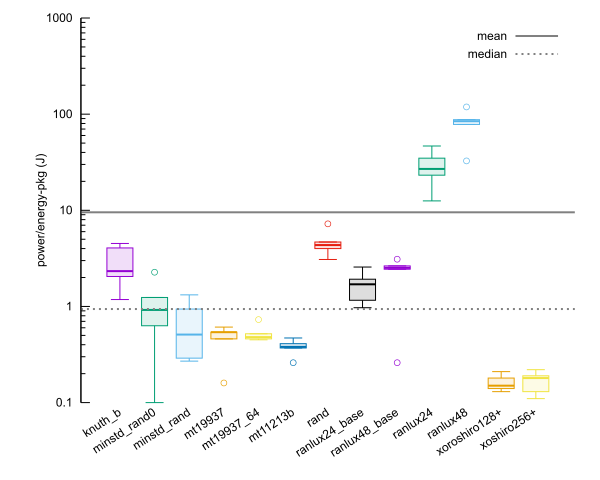
\includegraphics[width=\linewidth]{pkg.png}
\caption{Energy consumption of C++ standard RNGs.}
\label{fig:pkg}
\end{figure*}

\begin{figure*}
\centering
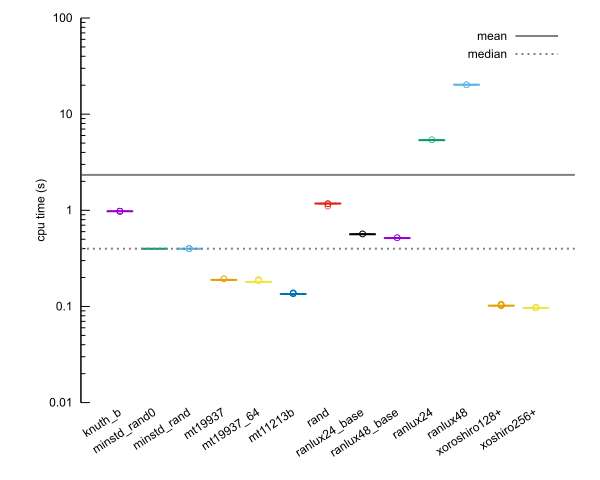
\includegraphics[width=\linewidth]{cpu.png}
\caption{CPU time spent by C++ standard RNGs.}
\label{fig:cpu}
\end{figure*}

% \begin{figure}
% \centering
% 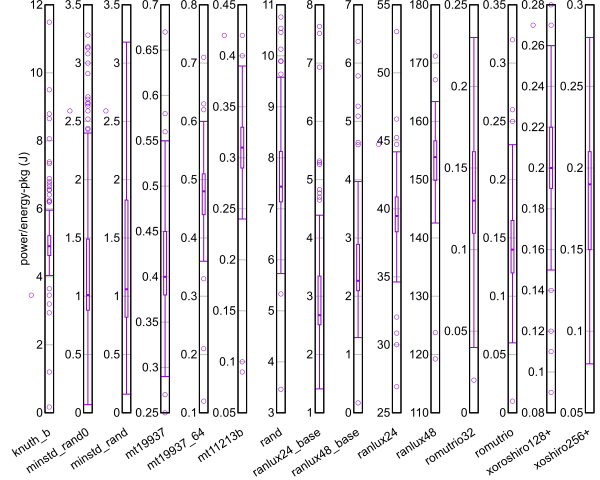
\includegraphics[width=\linewidth]{all.png}
% \caption{Energy consumption of C++ standard RNGs.}
% \label{fig:all}
% \end{figure}

In our case, the 32 bits version of \texttt{romutrio}, \texttt{romutrio32}, is the most efficient in terms of energy consumption and CPU time, while the \texttt{ranlux48} generator is the least efficient. The differences between the generators are also reflected in Table \ref{tab:pkg}, which shows the means and standard deviations of the energy consumed and the CPU time spent by 100 runs of each engine creating 100 million random numbers. \texttt{romutrio32} consume the 0.09\% of the energy consumed by \texttt{ranlux48} and the 0.41\% of the CPU time spent by \texttt{ranlux48}.

\begin{table}
\centering
\caption{Average energy consumption and CPU time, along with their standard deviations, for 100 runs of C++ standard RNGs producing 100 million random numbers.}
\begin{tabular}{lcc}
\toprule
Generator & Energy (J) & Time (s) \\
\midrule
knuth\_b & 5.1256$\pm$1.4059 & 0.9778$\pm$0.0004 \\
minstd\_rand0 & 1.3238$\pm$0.7541 & 0.3985$\pm$\textbf{0.0002} \\
minstd\_rand & 1.3379$\pm$0.8194 & 0.3985$\pm$\textbf{0.0002} \\
mt19937 & 0.4116$\pm$0.0693 & 0.1891$\pm$0.0007 \\
mt19937\_64 & 0.4770$\pm$0.0759 & 0.1806$\pm$0.0019 \\
mt11213b & 0.3068$\pm$0.0482 & 0.1349$\pm$0.0006 \\
rand & 7.6998$\pm$1.1038 & 1.1750$\pm$0.0075 \\
ranlux24\_base & 3.0864$\pm$1.1094 & 0.5636$\pm$0.0013 \\
ranlux48\_base & 2.5486$\pm$0.9063 & 0.5145$\pm$0.0009 \\
ranlux24 & 39.5458$\pm$3.1765 & 5.3631$\pm$0.0193 \\
ranlux48 & 153.1331$\pm$6.6647 & 20.2619$\pm$0.0232 \\
romutrio32 & \textbf{0.1357}$\pm$0.0340 & \textbf{0.0826}$\pm$0.0004 \\
romutrio & 0.1415$\pm$0.0405 & 0.0848$\pm$0.0005 \\
xoroshiro128+ & 0.2037$\pm$\textbf{0.0313} & 0.1021$\pm$0.0005 \\
xoshiro256+ & 0.1817$\pm$0.0379 & 0.0968$\pm$\textbf{0.0002} \\
\bottomrule
\end{tabular}
\label{tab:pkg}
\end{table}

After \texttt{romutrio32} and \texttt{romutrio}, the next best engines are the Mersenne Twister \texttt{mt11213b} and XOR based ones from Marsaglia, \texttt{xoroshiro128+}, and \texttt{xoshiro256+}, though not by a large margin.

Is also important to note that most of the implementations with lower energy consumption are 32 bits based, although their corresponding 64 bits versions are not much worse. As we can see when comparing a couple of examples:
\begin{itemize}
\item \texttt{mt19937\_64}, the 64 bits version of \texttt{mt19937}, consumes 15.89\% more energy and -4.49\% less CPU time.
\item \texttt{romutrio}, the 64 bits version of \texttt{romutrio32}, consumes 4.27\% more energy and 2.66\% less CPU time.
\end{itemize}

The energy consumption of the classic C \texttt{rand} generator is also very high, which is consistent with its poor performance in terms of CPU time. In spite of being one of the 32 bits implementations.

As a curious case, we can highlight \texttt{mt11213b}, one of the Mersenne Twister family generators. Its characteristics are among the best, and the only thing that differentiates it from \texttt{mt19937} is the set of constants and initial seeds. However, \texttt{mt11213b} consumes 34.16\% less energy and 40.18\% less CPU time than \texttt{mt19937}.

In our experiments, a perfect correlation has been found between energy consumption and CPU time used, with the most energy-efficient generators also being the fastest. This is easy to see by comparing figures \ref{fig:pkg} and \ref{fig:cpu}.

Both the code for the pseudo-random number generators implemented here and the code for the experiments conducted are available in the repository \url{https://github.com/gstvrmrlpz/energy}.

\section{Conclusions}
\label{sec:conclusions}

This study highlights significant disparities in energy consumption among various C++ standard RNGs, revealing a difference of over three orders of magnitude between the most efficient generator, \texttt{romutrio32}, and the least efficient, \texttt{ranlux48}, with the latter consuming exactly $1130.96$ times more energy. This disparity has substantial implications for applications that require the generation of large volumes of random numbers, such as artificial intelligence, genetic algorithms, and other computational tasks with heavy random number usage.

In conclusion, the significant variation in energy consumption among C++ standard RNGs not only emphasizes the importance of careful selection in algorithm design but also points to the need for a broader awareness of energy implications in software development practices. This research contributes to the growing discourse on green computing, encouraging ongoing efforts to develop energy-efficient algorithms and systems.

As future work, it would be interesting to replace, where possible, the RNG in the genetic algorithm libraries mentioned in Section \ref{sec:state-of-the-art} to analyze its impact on energy efficiency. Since random number generation takes up a large percentage of the execution time of evolutionary algorithms, the choice of an efficient generator should have a significant impact on the energy consumption of these algorithms.

\begin{acks}
This work is supported by PID2023-147409NB-C21 and PID2020-115570GB-C22 projects funded by MICIU/AEI/10.13039/501100011033 (Ministerio Español de Ciencia, Innovación y Universidades), as well as C-ING-027-UGR23 project, funded by ERDF/EU.
\end{acks}

\bibliographystyle{ACM-Reference-Format}
\bibliography{std-gecco-poster-2025}

\end{document}
